\chapter{Modelo matemático}

De acuerdo con \cite[p.~14]{Dombre2007}, el diseño y control de robots requiere diversos modelos matemáticos, tales como:

\begin{itemize}
\item Cinemática directa e inversa, es decir, encontrar la posición del efector final en términos de las coordenadas de las articulaciones y viceversa.
\item Cinemática de la velocidad, encontrar la velocidad del efector final en términos de la velocidad de las articulaciones y viceversa.
\item Modelo dinámico, el cual establece la relación entre los torques o fuerzas que ejercen los actuadores y las posiciones, velocidades y aceleraciones de las articulaciones.
\end{itemize}

\begin{figure}
    \centering
    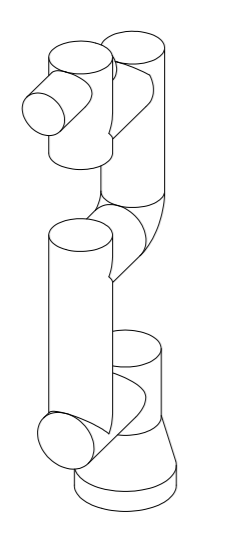
\includegraphics[scale=0.7]{./img/chapter4/robotarmprototype.png}
    \caption{Boceto del brazo robótico propuesto}
    \label{fig:roboticarmprototype}
\end{figure}

En este capítulo se desarrollarán los modelos matemáticos necesarios para simular y diseñar el brazo robótico, así como predecir el comportamiento del mismo.

Para realizar estos modelos, es importante contar con los parámetros físicos y geométricos del robot, los cuales aún no están completamente definidos, por lo que, en una primera aproximación, se mencionan en la tabla \ref{table:parametrosbrazorobotico}.



\begin{table}
\centering
\caption{Parámetros del brazo robótico}
 \label{table:parametrosbrazorobotico}
\begin{tabular}{l|l|l|l|l|l|l|}
                       & Eslabón 1   & Eslabón 2   & Eslabón 3   & Eslabón 4   & Eslabón 5   & Eslabón 6    \\ 
\hline
Longitud [m]           & 0.152       & 0.104       & 0.244       & 0.104       & 0.213       & 0.104        \\
Masa [kg]              & 0           & 2           & 1           & 0.8         & 0.8         & 0.2          \\
Centro de gravedad [m] & {[}0, 0, 0] & {[}0, 0, 0] & {[}0, 0, 0] & {[}0, 0, 0] & {[}0, 0, 0] & {[}0, 0, 0]  \\
Matriz de inercia      & {[}0, 0, 0] & {[}0, 0, 0] & {[}0, 0, 0] & {[}0, 0, 0] & {[}0, 0, 0] & {[}0, 0, 0]  \\
Fricción en eslabón    & 0.00148     & 0.00817     & 0.00138     & 7.12e-05    & 8.26e-05    & 3.67e-05     \\
Fricción de Coulomb    & 0.395       & 0.126       & 0.132       & 0.0113      & 0.00926     & 0.00396      \\
Inercia del motor      & 0.002       & 0.002       & 0.002       & 3.3e-05     & 3.3e-05     & 3.3e-05     
\end{tabular}
\end{table}

Otros requerimientos necesarios para el desarrollo del modelo matemático es el alcance total del brazo, el cual deberá ser de mínimo 500 mm, la velocidad, la cuál deberá estar en un rango entre 5 RPM y 30 RPM, y por último, la carga útil deberá ser de 2 kg.

En la figura \ref{fig:roboticarmprototype} podemos ver un boceto del brazo robótico que se planea implementar.

Con estos datos claros, es posible empezar la realización de los modelos matemáticos.

\section{Cinemática directa e inversa}
\subsection{Cinemática directa}

La cinemática directa de un robot se refiere al cálculo de la posición y orientación del marco de referencia del efector final a partir de las coordenadas $\theta$ de sus articulaciones. \cite{University2017}

\subsubsection{Matriz de transformación homogénea}

Según \cite{University2017}, existen tres usos principales para una matriz de transformación homogénea:

\begin{enumerate}
  \item Para representar la configuración (posición y orientación) de un cuerpo rígido.
  \item Para cambiar el marco de referencia en el cuál está representado un vector o un \textit{frame}.
  \item Para desplazar un vector o un \textit{frame}.
\end{enumerate}

Para el caso que nos ocupa, necesitamos la matriz de transformación homogénea desde la base fija del robot hasta su efector final, descrita con la ecuación siguiente:

\begin{equation}
\label{eq:homogeneustransformationmatrix}
\begin{split}
{}_{0}^{7}T = \mathscr{T}_z(a_1)\oplus\mathscr{R}_z(\theta_1)\oplus\mathscr{T}_x(b_1)\oplus\mathscr{R}_x(\theta_2)\oplus\mathscr{T}_z(c_1)\oplus\mathscr{R}_x(\theta_3) \\ \oplus\mathscr{T}_z(d_1)\oplus\mathscr{T}_x(d_2)\oplus\mathscr{R}_x(\theta_4)\oplus\mathscr{T}_x(e_1)\oplus\mathscr{R}_z(\theta_5)\oplus\mathscr{T}_z(f_1)\oplus\mathscr{R}_x(\theta_6)
\end{split}
\end{equation}

\begin{figure}
    \centering
    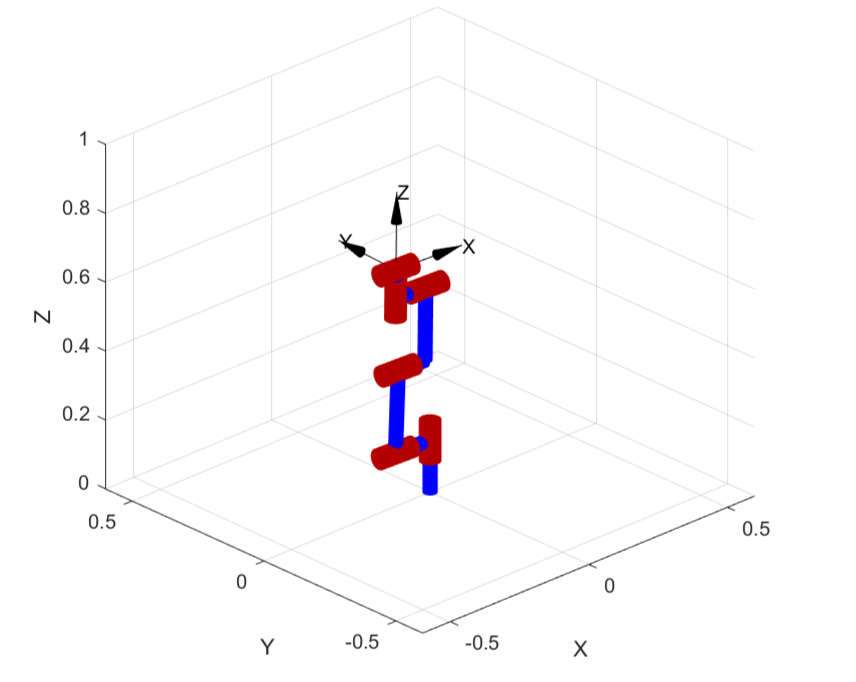
\includegraphics[scale=0.6]{./img/chapter4/KinematicDiagramML.png}
    \caption{Cadena cinemática}
    \label{fig:kinematicchain}
\end{figure}


En la imagen \ref{fig:kinematicchain} podemos observar la cadena cinemática de nuestro brazo robótico, fue creada con un algoritmo en MATLAB con ayuda de la herramienta Robotic Toolbox, desarrollada por Peter Corke \cite{Corke2017}, dicho código puede consultarse en el Anexo 1.


\subsubsection{Convención de Denavit-Hartenberg}

En muchas aplicaciones, es necesario representar los parámetros cinemáticos de forma simplificada con ayuda de la notación Denavit-Hartenberg, con esta, podemos hacer uso de algoritmos de solución para encontrar los valores dinámicos, planeación de trayectorias, simulaciones, entre otras.

Peter Corke \cite{Corke2007} propuso un acercamiento sencillo y sistemático para convertir una matriz de transformación homogenea como la de la ecuación \ref{eq:homogeneustransformationmatrix} en los parámetros de Denavit-Hartenberg. 

Se realizó dicho proceso con ayuda de Robotic Toolbox del mismo autor y se llegó a los resultados que se muestran en la tabla \ref{table:denavithartenberg}.

\begin{table}[h]
\centering
\caption{Parámetros Denavit Hartenberg}
 \label{table:denavithartenberg}
\begin{tabular}{l|l|l|l|l|}
               & $\theta$ [rad] & d [m]    & a [m]   & $\alpha$ [rad]                        \\ 
\hline
Articulación 1 & $\theta_1$              & 0.152    & 0       & $\frac{\pi}{2}$   \\
Articulación 2 & $\theta_2$              & 0        & -0.244       & 0 \\
Articulación 3 & $\theta_3$                  & 0 & -0.213       & 0                                                  \\
Articulación 4 & $\theta_4$              & -0.012        & 0 & $-\frac{\pi}{2}$   \\
Articulación 5 & $\theta_5$                        & 0.085        & 0 & $\frac{\pi}{2}$  \\
Articulación 6 & $\theta_6$                           & 0        & 0  & $-\frac{\pi}{2}$                                                 
\end{tabular}
\end{table}

\subsection{Cinemática inversa}

De manera parecida a como se manejó en la sección anterior, la librería de Robotic Toolbox tiene un método establecido para calcular la cinemática inversa dada una matriz de transformación homogénea.

En este texto se hará uso de la misma y no se abordará en mayor profundidad. 

\section{Cinemática de la velocidad}


\section{Modelo dinámico}

Como se comentó al principio del capítulo, es necesario establecer una relación entre las posiciones, velocidades y aceleraciones deseadas y el torque o fuerzas que se debe ejercer en los actuadores, esto nos permitirá controlar el brazo robótico así como conocer los parámetros necesarios que los actuadores deben cumplir para satisfacer los requerimientos de velocidad y carga útil.


\subsection{Formulación Newton-Euler}

Para el desarrollo del modelo dinámico se favoreció la formulación de Newton-Euler en lugar de la formulación Lagraniana, esto debido a su eficiencia computacional.

Para encontrar los torques a los que deben estar sometidos las articulaciones del brazo robótico se utilizará la herramienta que se ha utilizado a lo largo de este capítulo, Robotic Toolbox de Peter Corke, se desarrolla un algoritmo en MATLAB donde se incluiyen los parámetros necesarios para el modelo dinámico tales como masa, centro de gravedad, momento de inercia, fricción viscosa, fricción de Coulomb, inercia del motor y relación de engranes. 

La lista de parámetros para cada articulación y eslabón fue descrita anteriormente en el cuadro \ref{table:parametrosbrazorobotico}.

Cabe destacar que algunos de los parámetros dinámicos son una aproximación optimista, al no tener aún un diseño final ni todos los componentes seleccionados, sin embargo, es funcional para una primera iteración del torque necesario para empezar la selección de componentes.

Con los datos del cuadro \ref{table:parametrosbrazorobotico} se selecciona los torques máximos en el escenario más demandante, esto es en una trayectoria en la cuál cada una de las articulaciones se somete a una mayor fuerza.

Con todos los datos correctamente particularizados, obtenemos una lista con todos los valores máximos, se puede apreciar en el cuadro \ref{table:maxtorque}. 

\begin{table}[h]
\centering
\caption{Torque máximo por articulación}
\label{table:maxtorque}
\begin{tabular}{l|l|l|l|l|}
               & $\theta$ [rad] & d [m]    & a [m]   & $\alpha$ [rad]                        \\ 
\hline
Articulación 1 & $\theta_1$              & 0.152    & 0       & $\frac{\pi}{2}$   \\
Articulación 2 & $\theta_2$              & 0        & -0.244       & 0 \\
Articulación 3 & $\theta_3$                  & 0 & -0.213       & 0                                                  \\
Articulación 4 & $\theta_4$              & -0.012        & 0 & $-\frac{\pi}{2}$   \\
Articulación 5 & $\theta_5$                        & 0.085        & 0 & $\frac{\pi}{2}$  \\
Articulación 6 & $\theta_6$                           & 0        & 0  & $-\frac{\pi}{2}$                                                 
\end{tabular}
\end{table}


  